\documentclass[12pt,a4paper,twoside]{article}
\usepackage{a4wide}
\usepackage[slovene]{babel}
\usepackage[utf8]{inputenc}
\usepackage[T1]{fontenc}
\usepackage{epsfig}
\usepackage{subfigure}
\usepackage{fancyhdr}
\usepackage{hyperref} %za spletne povezave

\usepackage{tikz} %za tabele
\usetikzlibrary{matrix}%za tabele


\begin{document}
\baselineskip 19pt \thispagestyle{empty}

%%*
\begin{center}
%{\large Osnovna šola Mokronog}\\ 
{\Huge\bf Linux notes}\\
[1cm] {\large \bf zapiski za pomoč pri delu v OS Linux}\\



\begin{figure}[h!] \centering
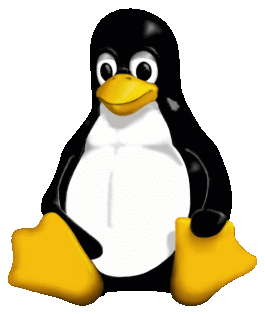
\epsfig{file=slike/Tux.png, angle=0,clip=, width=6cm}
%\caption{}\label{slika:tux}
\end{figure}


 Avtor: Tomaž Kušar


Mokronog, marec 2019\linebreak 

\begin{figure}[h!] \centering

\epsfig{file=slike/CC_koda.png,angle=0}
\end{figure}

\end{center}
%\newpage
\clearpage \setcounter{page}{2}
\newpage


\noindent \textbf{Povzetek}\\
V skripti so razni zapiski, s katerimi si lahko pomagate pri delu v OS Linux. Predvsem so napotki vezani na distribucijo Bunsenlabs, seveda pa ukazi delujejo tudi na drugih distibucijah z snovo debian.


\newpage

\tableofcontents
\newpage
\pagestyle{fancy}
\renewcommand{\sectionmark}[1]{\markright{T. Kušar. Delam z Linux-om }}
\renewcommand{\subsectionmark}[1]{\markright{T. Kušar. Delam z Linux-om }}
\renewcommand{\subsubsectionmark}[1]{\markright{T. Kušar. Delam z Linux-om }}

\section{Linux da ali ne?}
To skripto sem napisal predvsem zato, da si izdelam zapiske, kako si urediti računalnik z OS Linux. Ker sem  na Linux-ih pravzaprav pravi začetnik (resni in redno jih uporabljam dobra tri leta), je v skripti opisano mnogo stvari, od samega začetka pa tudi do bolj kompliciranih zadev, v splošnem pa je v skripti tisto, kar sem zares potreboval. Najprej pa moram odgovoriti na pomisleke, zakaj je smiselno na računalnik namestit OS Linux.

\begin{itemize}
\item OS je prostodostopen in zanj ni potrebno plačati od 100 do 200 evrov in vse je uradno.
\item Za računalnik ni potrebno iskat gonilnikov. Namestitev je zelo enostavna. 
\item Na računalniku ne potrebujemo protivirusnega programa, saj je virusov za OS Linux zelo malo.
\item Obstajajo distribucije Linuxa (s podporo!), ki delujejo na starejših računalnikih. Ena izmed njih je distribucija Bunsenlab. Obstajajo pa še druge kot na primer Linux Lubuntu, Xbuntu, Puppy Linux.
\item Posodobitev namestimo ko hočemo. Samodejnih posodobitev ni. Tako se nam ni treba ukvarjati s posodobitvami, ko se nam najbolj mudi. 
\item Ni potrebno posebej omenjati, da vse deluje zelo hitro.
\item Zaradi široke mreže uporabnikov, se tudi napake in hrošči hitro odpravljajo. Težave se torej hitro rešijo in ni potrebno čakati na varnostne posodobitve. Seveda pa so že v osnovi "pingvini" bolj varni od "oken". 
\end{itemize}

Zakaj pa Lunuxa nebi imeli? 
No, če smo odvisni od pisarniškega paketa Microsoft Office, potem bo prehod na linux malce težak. Pravzaprav bodo težave, če imamo kakršenkoli poseben program, ki obstaja samo za OS Windows. Sicer pa za vsa področja najdemo programe, ki delujejo na OS Linux. Da ne bo pomote. Tudi sam sem še zmeraj trenutno odvisen od "oken", večino zadev pa vendarle naredim na pingotih.

\newpage
\section{Programi za OS Linux}
V tabeli so navedeni alternativni programi po mojem izboru, ki nadomestijo vse najpogosteje uporabljene programe za obdelavo slik, videa, zvoka, pisarniških programov in raznih pripomočkov. Skrb, da česa ne bi mogli urediti je praktično odveč.

\tikzset{ 
    table/.style={
        matrix of nodes,
        row sep=-\pgflinewidth,
        column sep=-\pgflinewidth,
        nodes={
            rectangle,
            draw=black,
            align=center
        },
        minimum height=3.2em,
        text depth=0.5ex,
        text height=0ex,
        nodes in empty cells,
%%
        every even row/.style={
            nodes={fill=gray!20}
        },
        column 1/.style={
            nodes={text width=2em,font=\bfseries}
        },
        row 1/.style={
            nodes={
                fill=black,
                text=white,
                font=\bfseries
           }
        }
    }
}

\begin{tikzpicture}

\matrix (first) [table,text width=4.5cm]
{
& Področje   & Windows & Linux \\
1 & Urejanje besedil   & Word (MS Office) & Writer (Libre Office)\\
2 & Urejanje fotografij   & Photoshop & Gimp\\
3 & Vektorska Slika   & Corel Draw & Inkscape \\
4 & Video   & Movie Maker & Open Shot, KDenLive \\
5 & LaTex besedila & Texmaker & Texmaker\\
6 & Urejanje tekstovnih datotek & Sublime text & Sublime text\\
7 & 3D modeliranje & SketchUp FreeCad & FreeCad, OnLine SketchUp\\
8 & CAD načrtovanje & QCAD & QCAD\\
9 & Odpiranje PDF dokumentov & Adobe Reader & Foxit Reader\\
10 & Poštni odjemalec & Outlook & Thunderbird\\
11 & Urejanje zvočnih datotek & Audacity & Audacity\\
12 & Digitalna preslikava dokumentov & Programska oprema skenerja & Xsane\\
};
\end{tikzpicture}




\newpage
 %\pagestyle{myheadings} \markright {\underline{\mbox{"
%"}T.Kušar.Uporaba mikrokrmilnika pri brezžièni
%komunikaciji.Diplomsko delo \mbox{"     "}}}


\section{Namestitev}
%
%\begin{figure}[h!]
%\centering
%\epsfig{file=Slike/komunikacija.jpg,angle=0,clip=,width=8cm}
%\caption{Model komunikacije.}\label{slika:Komunikacija}
%\end{figure}
%

Linux distribucij je mnogo. Katero izbrati, je stvar potrebe. Če imamo starejši računalnik, potem je smiselno poiskati distribucijo, ki podpira tudi starejše arhitekture računalnika. In prav takšna distribucija je opisana v teh navodilih. V našem primeru sem izbral linux BunsenLab. Omenjeno distribucijo najdemo na naslovu \href{https://www.bunsenlabs.org/}{bunsenlab}. Omenjen operacijski sistem je zasnovan na osnovi Debian, tako da je v nadaljevanju potrebno iskati programe za sistem Debian. 

Veliko bolj popularen je sicer operacijski sistem Linux Ubuntu, ki ga najdemo v različnih verzijah (MATE, MINT ...)

Namestitev je enostavna. Ustvarimo si namestitveni CD, ali namestitveni USB ključek. Navodila najdete na spletu oziroma na spletni strani, kjer si presnamete operacijski sistem. Sledite navodilom in namestite sistem. Če želite imeti na računalniku poleg OS Linux še OS Windows, pa je potrebno razdeliti disk na dve particiji z ustreznim programom. Pri starejših računalnikih ne bo problema, pri novejših pa se stvar dodatno zaplete, saj imajo v BIOS-u varnostne nastavitve. Potrebno je poiskati navodila na spletu (ključne besede: UEFI, security boot).  Torej, ustvariti si morate dual boot.

%\begin{figure}[h!] \centering
%\epsfig{file=Slike/rtfq1shema.jpg,angle=0,clip=,width=6cm}
%\caption{Shema radijskega oddajnega modula.}\label{slika:rtfq1shem}
%\end{figure}

\section{Namestitev antivirusnega programa}
Ja, tudi na OS Linux lahko namestimo protivirusni program, saj obstajajo tudi virusi za OS linux - čeprav manj pogosto. S spletne strani si lahko presnamemo program Comodo in sicer .deb paket. Potem pa ga odpakiramo z ukazom:


 \texttt{sudo dpkg -i \textless file\_name\textgreater.deb}

Sledimo navodilom, ki se izpišejo v terminalu. Pognati moramo datoteko \texttt{post\_setup.sh} v mapi \texttt{/opt/COMODO.}


%\begin{figure}[h!] \centering
%\epsfig{file=Slike/anteneshem.jpg,angle=0,clip=,width=6cm}
%\caption{Shema radijskih anten. Zgoraj spiralna, spodaj navadna
%\cite{rfstran}.}\label{slika:antene}
%\end{figure}

\section{Namestitev datuma in ure}
Uro in datum nastavimo v terminalnem oknu z ukazom:

\texttt{timedatectl set-time '2017-04-22 7:34:00'}

Če želimo nastaviti samo uro uporabimo ukaz:

\texttt{ date +\%T -s "10:23:00"}

Ja, ta ukaz pride prav, saj nam ni potrebno odpirati oken in podoken... Enostavno to uredimo preko terminala. 

\section{Namestitev tiskalnika in optičnega čitalnika}
Namestitev navadnega tiskalnika ni zahtevna. Največkrat zadostuje, da namestimo podporo za tiskalnike v BL meniju. 

\begin{figure}[h!] \centering
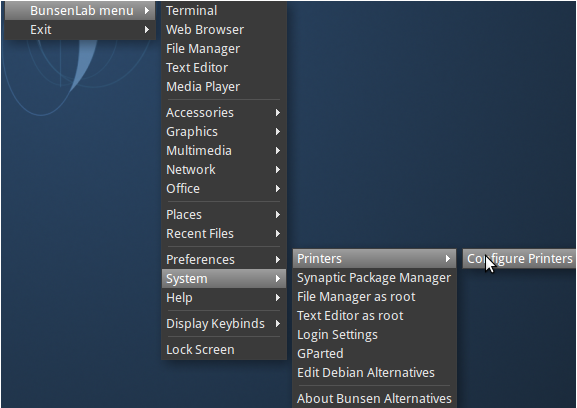
\epsfig{file=slike/printer_setup.png,angle=0,clip=,width=6cm}
\caption{Nastavitve tiskalnika v meniju BL
\cite{rfstran}.}\label{slika:Nastavitve tiskalnika v meniju BL}
\end{figure}

Za namestitev optičnega čitalnika je potrebno namestiti najprej programsko opremo. Imamo več možnosti. Izbral sem program XSANE, ki ga namestimo z ukazom:


\texttt{sudo apt-get install sane sane-utils libsane-extras xsane}


Z ukazom \texttt{sudo sane-find-scanner} hitro preverimo, če program najde ustrezno strojno opremo. V mojem primeru sem potreboval še dodatne pakete za HP tiskalnik oziroma optični čitalec: \texttt{sudo hp-setup}. Tu gre vsa zahvala podjetju HP, ki je poskrbelo za gonilnega njihovih tiskalnikov za OS Linux. S HP tiskalniki torej na Linuxih ne bo težav.



\section{Dodajanje uporabnika}

\texttt{sudo useradd -m imeuporabnika}\linebreak 
\texttt{sudo passwd imeuporabnika}\linebreak 
\texttt{sudo usermod -s /bin/bash imeuporabnika}



\newpage
\section{Namestitev programa Wink za izdelavo interaktivnih gradiv}

S spleta presnamemo mapo wink15\_b1060.tar.gz. Odtaramo jo v mapo opt in poženemo inštalacijsko datoteko:

\texttt{sudo tar -C /opt -xf wink15\_b1060.tar.gz}

\texttt{cd /opt}

\texttt{./installer.sh}

Sitem bo najbrž javil, da manjkata dve knjižnici in sicer libstdc++.5 in libexpat.so.0. To prvo lahko poiščemo preko synaptic paketov. Ni nujno da izberemo ravno tisto različico libstdc, lahko tudi novejšo. S to drugo knjižnico bodo težave. Lahko namestimo preko paketov podobne knjižnice. Sicer pa namestimo:


\texttt{sudo apt-get install libexpat-dev:i386}

Potem pa preimenujemo knjižnico:

\texttt{sudo ln -s /lib/i386-linux-gnu/libexpat.so.1 /lib/i386-linux-gnu/libexpat.so.0}

\textbf{OPOMBA}: Ker je program wink za linux malce težje najti na spletu, sem ga skopiral na svojo spletno stran. obstaja pa še ena težava in sicer, program WINK za Linux obstaja samo za 32-bitno različico. Na 64-bitnem sistemu winka ne bomo mogli namestiti.



\begin{figure}[h!] \centering
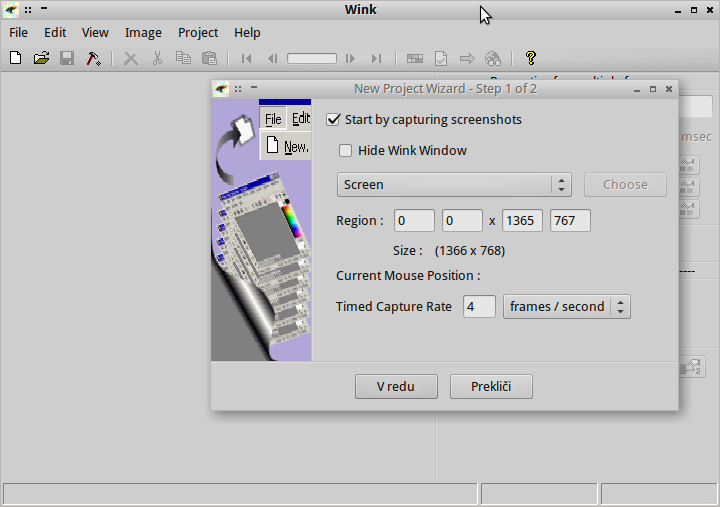
\epsfig{file=slike/wink.png,angle=0,clip=,width=10cm}
\caption{Okno programa Wink}\label{slika:Okno programa WInk}
\end{figure}

\subsection{Izdelava bližnjice za program Wink}

Inštaliramo si paket:

\texttt{sudo apt-get install  "--no-install-recommends gnome-panel}

Potem pa ta gnome panel poženemo:

\texttt{sudo gnome-desktop-item-edit  $\sim$/Desktop/ "--create-new}

Pokaže se vnosno okno, kamor vpišemo oziroma pokažemo pot do datoteke, ki jo želimo zagnati. 

\begin{figure}[h!] \centering
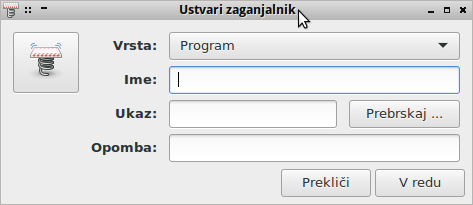
\epsfig{file=slike/gnome_desktop_edit.png,angle=0,clip=,width=10cm}
\caption{Gnome desktop edit}\label{slika:Gnome desktop edit}
\end{figure}

Ko pokažemo na datoteko, se nam v mapi Desktop ustvari desktop datoteka. 

\begin{figure}[h!] \centering
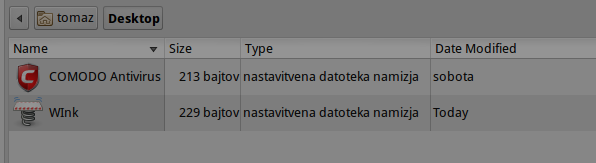
\epsfig{file=slike/desktop_wink.png,angle=0,clip=,width=10cm}
\caption{Wink datoteka}\label{slika:Wink datoteka}
\end{figure}

Postavimo se v mapo Desktop in kopiramo datoteko WInk.desktop v mapo /usr/share/applications:

\texttt{sudo cp WInk.desktop /usr/share/applications/WInk.desktop}

Da se v meniju ustvari ikona (povezava) v ustrezni kategoriji, dopišemo še parameter Categories datoteko:

\#!/usr/bin/env xdg-open\linebreak 
\[Desktop Entry\]\linebreak 
Version=1.0\linebreak 
Type=Application\linebreak 
Terminal=false\linebreak 
Icon[sl\_SI]=gnome-panel-launcher\linebreak 
Name[sl\_SI]=WInk\linebreak 
Exec=/opt/wink/wink\linebreak 
Name=WInk\linebreak 
Icon=gnome-panel-launcher\linebreak 
Categories=AudioVideo;Player;Recorder\linebreak 


\section{Povezava na skupno mapo}
Opisan je postopek, kako se povežemo na mapo, ki je na nekem drugem računalniku z OS Linux (samba share). Na računalnik si namestimo program Gigolo:

\texttt{sudo apt-get install gigolo}

Zaženemo program in dodamo zaznamek. Vpisati moramo IP računalnika in ime mape, ki je deljena. Seveda moramo vpisati tudi up. ime in geslo, na katerem je ta mapa.

\begin{figure}[h!] \centering
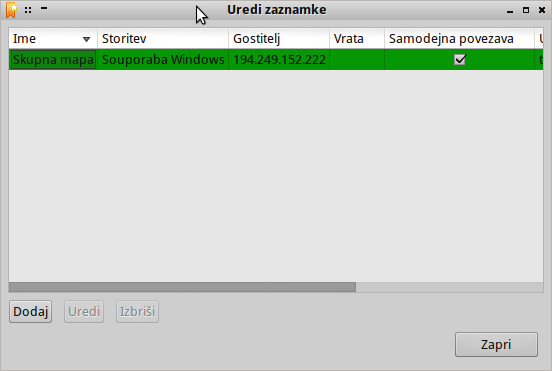
\epsfig{file=slike/gigolo_uredi_zaznamke.png,angle=0,clip=,width=10cm}
\caption{Dodajanje zaznamka}\label{slika:Dodajanje zaznamka}
\end{figure}

\begin{figure}[h!] \centering
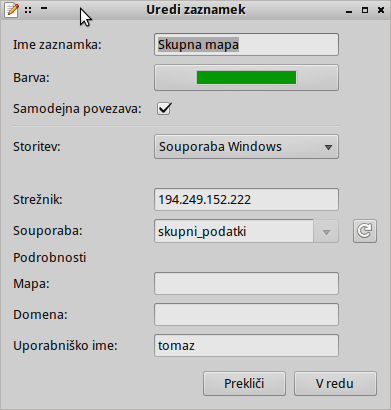
\epsfig{file=slike/gigolo.png,angle=0,clip=,width=7cm}
\caption{Nastavitev zaznamka za deljeno mapo}\label{slika:Nastavitev zaznamka za deljeno mapo}
\end{figure}

\begin{figure}[h!] \centering
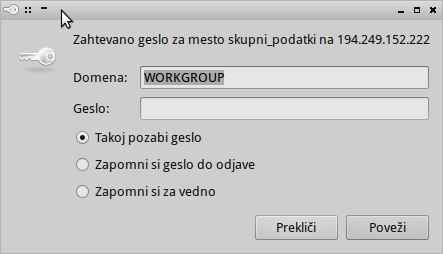
\epsfig{file=slike/gigolo_geslo.png,angle=0,clip=,width=7cm}
\caption{Povezava z mapo}\label{slika:Povezava z mapo}
\end{figure}

\newpage
\section{Urejanje video posnetkov}

Za urejanje video posnetkov si namestimo program kdenlive

\texttt{sudo apt-get install kdenlive}


\begin{figure}[h!] \centering
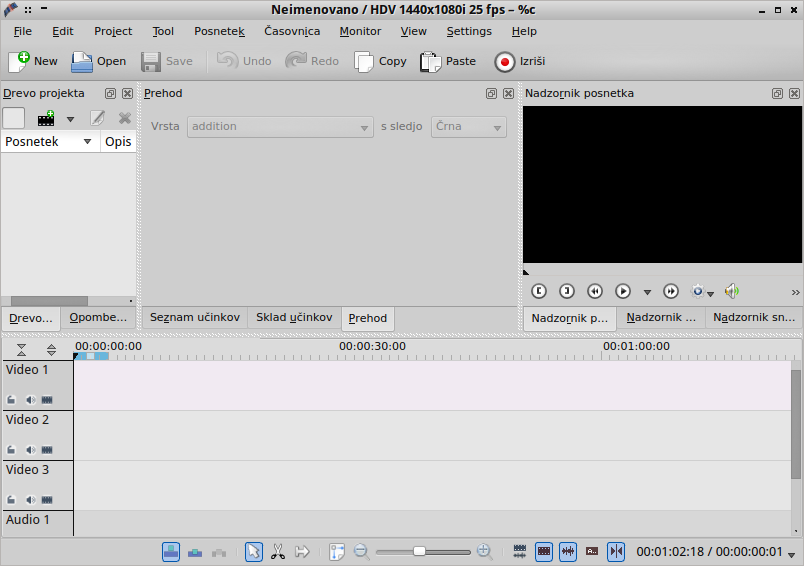
\epsfig{file=slike/kdenlive.png,angle=0,clip=,width=7cm}
\caption{Program Kdenlive za urejanje videoposnetkov}\label{slika:Program Kdenlive za urejanje videoposnetkov}
\end{figure}



\newpage
\section{Izvoz .tex datoteke v HTML}
Postavimo se v mapo, kjer imamo izvorno .tex datoteko in poženemo ukaz:
\texttt{htlatex imedatoteke.tex}

\begin{figure}[h!] \centering
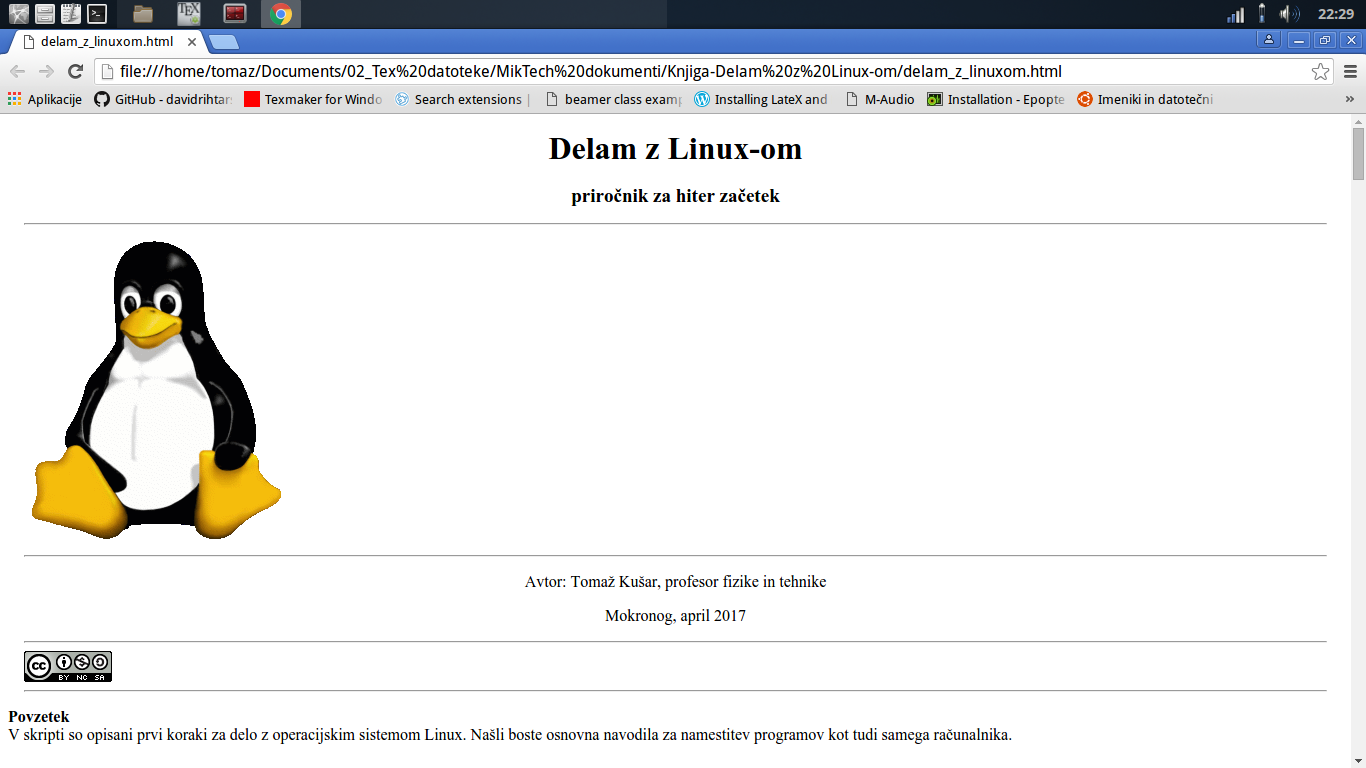
\epsfig{file=slike/tex_to_html.png,angle=0,clip=,width=17cm}
\caption{Skripta v HTML formatu}\label{slika:Skripta v HTML obliki}
\end{figure}


\section{Namestitev urejevalnika besedil Texmaker}
Texmaker je brezplačen, moderen LaTeX urejevalnik za OS Linux, MacOSX in OS Windows, ki združuje veliko orodij, potrebnih za razvoj dokumentov z lateksom v eni aplikaciji.
Texmaker vključuje podporo unicode, preverjanje črkovanja, samodejno dokončanje kode in vključuje sinhroniziran predogled dokumenta. Texmaker je enostaven za uporabo in konfiguracijo. Texmaker je izdan pod licenco GPL.

Namestitev je enostavna, traja pa kar nekaj minut! Ja minut, saj se mora namestiti precej paketov. Namestitev je najlažja preko terminalnega okna:

\texttt{sudo apt-get install texlive-full texmaker}

S tem namestimo texmaker z vsemi tex paketi in knjižnicami, ki jih pri delu potrebujemo. 

\subsection{Namestitev slovenskega črkovalnika}
Ko v tex-u pišemo besedilo, je smiselno da nas program samodejno opozarja na slovnične napake. Zato si moramo dodatno namestiti še slovenski slovar, ki je podlaga za popravljanje. 

Na spletu najdemo Slovenski črkovni slovar, Slovenian dictionary package (SLovenski pkaet slovarjev). Jaz sem našel slovar na strani http://extensions.services.openoffice.org/, katerega avtor je Martin Srebotnjak. Slovar je namenjen uvozu v OpenOffice. 

Presnamemo si datoteko \textbf{pack-sl.oxt}, ali nekaj podobnega. Postopek namestitve je naslednji. 

\begin{enumerate}
\item {Datoteki spremenimo končnico v .zip.}
\item {Odpakiramo zip datoteko}
\item {Potem pa vse skupaj skopiramo ali celotno mapo prestavimo nekam, kjer bomo imeli te slovarje in tex dokumente.} 
\item {Odpremo texmaker in v meniju izberemo Options \/ Configure Texmaker \/ in na levi kliknemo na urejanje Urejevalnika (Editor). V polju Spelling dictionary pokažemo pot do datoteke \textbf{sl\_SI.dic}, ki je v mapi.} 
\end{enumerate}

\begin{figure}[h!] \centering
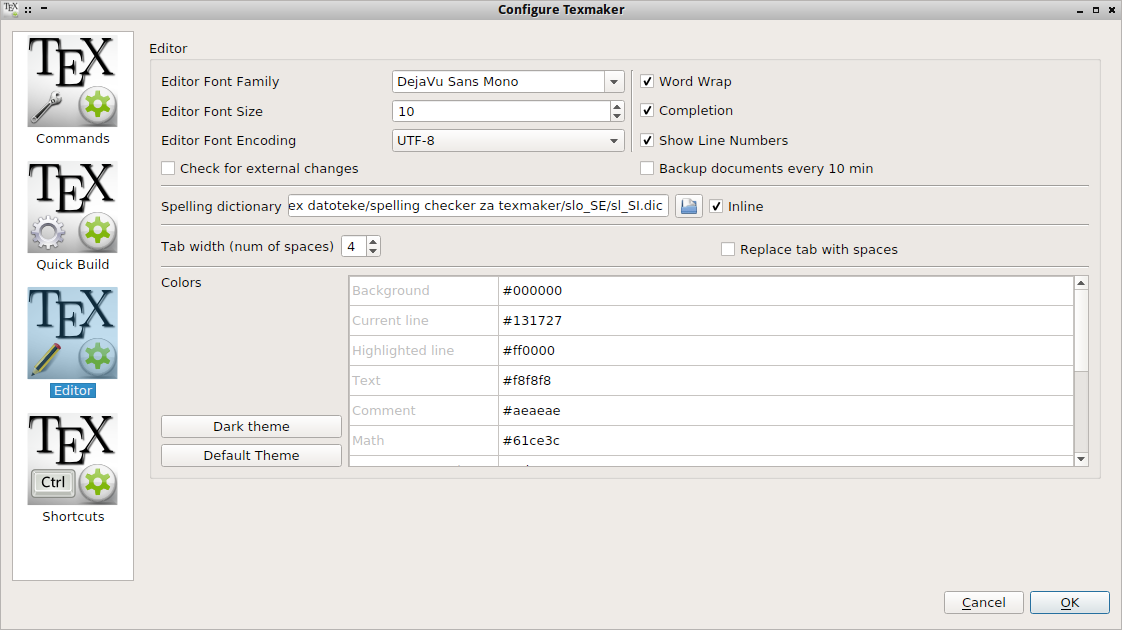
\epsfig{file=slike/spelling_dictionar_tex.png,angle=0,clip=,width=17cm}
\caption{Nastavitev slovenskega slovarja}
\label{slika:Nastavitev slovenskega slovarja}
\end{figure}

Ko potem ponovno zaženete texmaker, vam program samodejno podčrta predvidene napake. 

\subsection{Zakaj uporabljati texmaker?}
Dokumenti napisani v texu se enostavno prevedejo v pdf dokument, dokument pa je zelo profesionalen. Ni se nam potrebno ukvarjati z obliko dokumenta. 

\subsection{Texmaker na OS Windows}
Če oblikujete besedilno datoteko v tex-u, potem lahko dokument urejate tudi na OS Windows oziroma jo lahko prenesete na računalnik z OS Windows. Program Texmaker namreč deluje tudi na Windowsih. Je pa potrebno imeti nameščen paket MiKTeX (URL: https://miktex.org/download) in pa program texmaker (url: http://www.xm1math.net/tex maker/download.html). 


\newpage

\section{Zapis glasbe na CD}
Za zapis glasbe na zgoščenko lahko uporabimo več programov, na  primer Brasero ali pa K3b. Če pečemo CD s slednjim potem si lahko namestimo še dodatni paket, s katerim normaliziramo posnetke na zgoščenki. 

Ukaz za namestitev paketa je naslednji: 

\texttt{sudo apt-get install normalize-audio}


\section{Opis najbolj uporabnih programov}
V nadaljevanju je predstavljenih nekaj najbolj osnovnih programov ki jih potrebujemo pri vsakdanjem delu oziroma v šoli. Poudarek je na programih, ki se uporabljajo pri tehniki. 

\subsection{LibreOffice}
LibreOffice je brezplačni paket pisarniških programov. Vključuje Writer, Calc, Impress in druge. S programom Writer pišemo besedilne dokumente, program Calc je namenjen računanju in delu s podatki in tabelami, s programom Impress pa si izdelamo interaktivno predstavitev. 


\subsection{ArduinoIDE}
Arduino IDE je aplikacija za programiranje AVR mikrokrmilnikov v programskem jeziku C/C++. Je popolnoma brezplačna. 

\subsection{bCNC}
Je odprtokodna aplikacija z krmiljenje cnc naprav, na primer rezkarjev, tiskalnikov..., ki podpira GBRL standard. 

\subsection{Fritzing}
Je odprtokodni program za risanje elektrotehniških shem, pri če čemer lahko komponente vnašate tudi kot grafične objekte. 


\subsection{SublimeText}
Je program za urejanje tekstovnih datotek. Podpira razne programske jezike, tako da v njem lahko pišete tudi programsko kodo. 

\subsection{FileZilla}
FileZilla Client is a fast and reliable cross-platform FTP, FTPS and SFTP client with lots of useful features and an intuitive graphical user interface.

\subsection{GIMP}
Program za urejanje fotografij in slik, alternativa Photoshop-u. 

\subsection{Inkscape}
Program za urejanje in izdelavo vektorskih slik, alternativa CorelDraw-ju. 


\subsection{FoxitReader}
Pprogram za pregledovanje in urejanje PDF datotek, seveda brezplačen. 

\subsection{Kazam}
Pogosto pri sovojem delu potrebujemo zaslonsko sliko, ali del slike z zaslona, morda pa celo posnetek nekega opravila na računalniku. Vse to se da narediti s pomočjo programa kazam. 
Program namestimo z ukazom:

\texttt{sudo apt-get install kazam}

Začenemo pa ga prav tako v terminalnem oknu z ukazom:

\texttt{kazam}

\subsection{Stelarium}
Stelarium je program za ljubitelje astronomije, oziroma astronome in fizike. S programom je mogoče spremljati premikanje nebesnih teles (planetov, zvezd, meglic...) . Program prikazuje trenutno sliko neba, tudi podnevi. S klikom na posamezno nebesno telo, se nam izpiše na zaslonu ime izbranega telesa in osnovni  oziroma pomembni podatki. 

Namestitev: \texttt{sudo apt-get install stellarium }

\subsection{Tuxmath}
Tuxmath je program za učenje matematike. S programom se naučimo hitrega računanja. 


\subsection{GCompris}
Je didaktična igra, pravzaprav paket namenjena otrokom od 2 do 10 let. 
Namestitev-
      \texttt{sudo apt-get insall gcompris}
      
In potem si namestite še zvoke v slovenščini:

    \texttt{sudo apt-get install gcompris-sound-sl}

G Compris je paket didaktičnih iger za mlajše otroke. Učenci se naučijo klikati na miško, pisati s pomočjo tipkovnice, naučijo se klepetati v spletni klepetalnici, risati z računalnikom, reševati logične naloge, se učiti branja, pozornosti in še in še...

\begin{figure}[h!] \centering
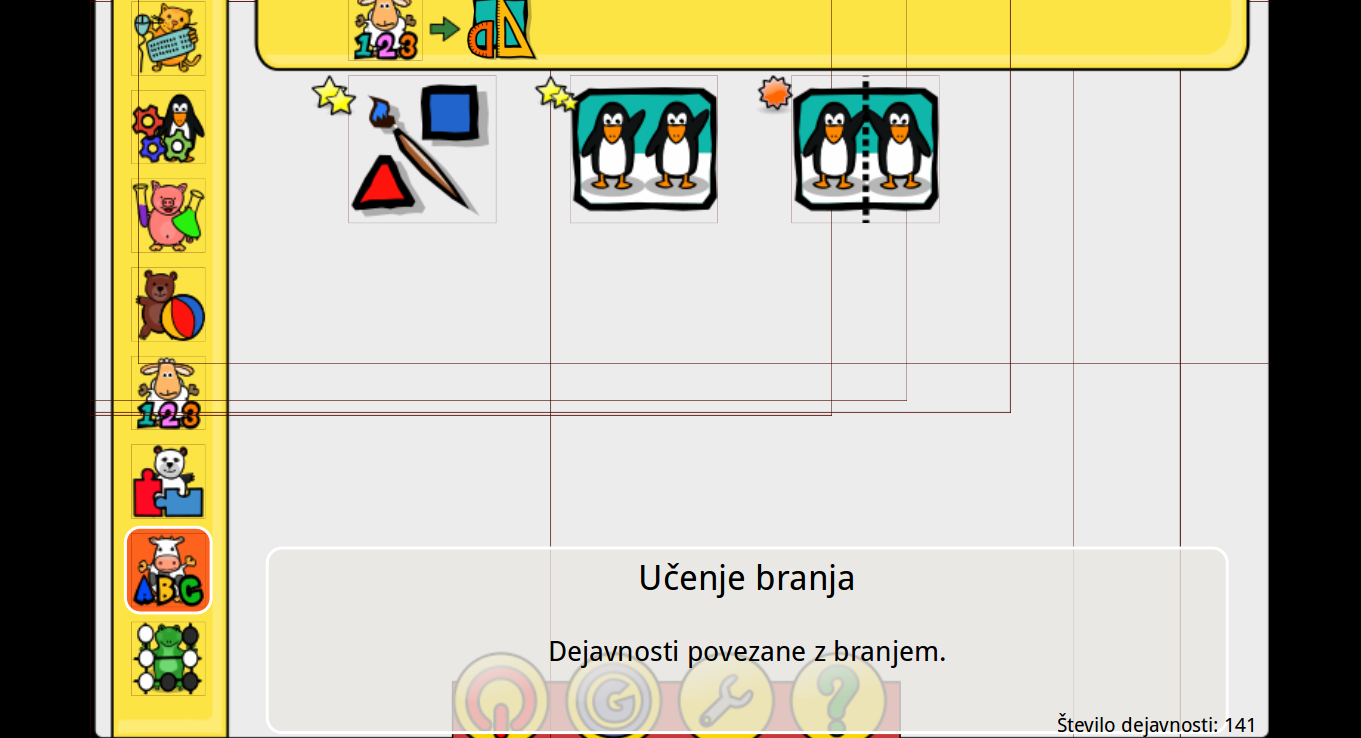
\epsfig{file=slike/gcompris.png,angle=0,clip=,width=17cm}
\caption{Okrno programa GCompris}
\label{slika:Okno programa GCompris}
\end{figure}


\subsection{Klavaro}
To je program namenjen učenju slepega tipkanja oziroma pravilnega tipkanja, kjer se uporabljajo vsi prsti. 

\subsection{SketchUp}
Program za 3D modeliranje. Na OS linux lahko 3D modeliramo s programom FreeCad ali pa spletno aplikacijo SkethUp. Če se prijavimo z Googlovim računom, potem lahko datoteke shranimo.

povezava do programa: https://app.sketchup.com


\end{document}
